\section{Experiments and Results}
\label{sec:experiments-results}

\subsection{Headline Quality: Golden and Held-Out States}
\label{sec:experiments-headline}

Tables~\ref{tab:detector-headline} and~\ref{tab:parser-headline} report the two
suites on all six states, four developed against and two held out entirely. All
numbers are on the \texttt{\_only\_subset} corpus tier (\S\ref{sec:corpus}),
never on full documents.

% AUTO-GENERATED by paper/analysis/generate_tables.py — do not hand-edit.
% Source: paper/results/task1_20260816/summary.json, task2_20260816/summary.json,
% corpus_tiers.json. Regenerate with: python paper/analysis/generate_tables.py
% Corpus tier (guardrail 1): every row is the _only_subset tier, never full-document.
\begin{table*}
  \centering
  \begin{tabular}{lrrrrrl}
    \hline
    \textbf{State} & \textbf{Role} & \textbf{Subset pp} & \textbf{Recall} & \textbf{Code acc.} & \textbf{Desc. acc.} & \textbf{Depth map} \\
    \hline
    AZ & golden & 15 & 100.0 & 100.0 (4/4) & 100.0 (4/4) & PASS \\
    CA & golden & 13 & 100.0 & 100.0 (25/25) & 100.0 (14/14) & PASS \\
    CO & golden & 10 & 100.0 & 100.0 (7/7) & 100.0 (4/4) & PASS \\
    TX & golden & 9 & 100.0 & 100.0 (8/8) & 100.0 (3/3) & PASS \\
    NV & held-out & 15 & 100.0 & 95.1 (39/41) & 66.7 (2/3) & PASS \\
    KY & held-out & 8 & 100.0 & 100.0 (44/44) & 100.0 (26/26) & PASS \\
    \hline
  \end{tabular}
  \caption{Detector recall, code and description accuracy, and depth-map pass/fail, per state. All numbers are on the \emph{\_only\_subset} corpus tier (8--15pp manually trimmed subsets; see \S\ref{sec:corpus}), never full documents. Golden = AZ/CA/CO/TX; held-out = NV-2023/KY. Source: \texttt{paper/results/task1\_20260816/}, \texttt{task2\_20260816/}.}
  \label{tab:detector-headline}
\end{table*}


% AUTO-GENERATED by paper/analysis/generate_tables.py — do not hand-edit.
% Source: paper/results/task1_20260816/summary.json, task2_20260816/summary.json,
% corpus_tiers.json. Regenerate with: python paper/analysis/generate_tables.py
% Corpus tier (guardrail 1): every row is the _only_subset tier, never full-document.
\begin{table*}
  \centering
  \begin{tabular}{lrrrrr}
    \hline
    \textbf{State} & \textbf{Role} & \textbf{Coverage} & \textbf{Field acc.} & \textbf{Standards} & \textbf{ID collisions} \\
    \hline
    AZ & golden & 100.0 (18/18) & 99.7 & 45 & 0 \\
    CA & golden & 100.0 (21/21) & 98.4 & 94 & 0 \\
    CO & golden & 100.0 (9/9) & 100.0 & 48 & 0 \\
    TX & golden & 100.0 (8/8) & 100.0 & 25 & 0 \\
    NV & held-out & 100.0 (15/15) & 97.4 & 24 & 0 \\
    KY & held-out & 100.0 (26/26) & 98.3 & 26 & 0 \\
    \hline
  \end{tabular}
  \caption{Parser coverage, per-field accuracy, standards emitted, and \texttt{standard\_id} collisions, per state. All numbers are on the \emph{\_only\_subset} corpus tier (\S\ref{sec:corpus}), never full documents. Golden = AZ/CA/CO/TX; held-out = NV-2023/KY. Source: \texttt{paper/results/task1\_20260816/}, \texttt{task2\_20260816/}.}
  \label{tab:parser-headline}
\end{table*}


\textbf{The precision column needs its definition stated.}
\emph{Verified precision} is (in-scope detections $-$ hallucinations) divided by
in-scope detections, taken from the manual false-positive audit: every unmatched
in-scope detection in all six states was examined and the verdict signed by the
author. I deliberately do not report the suites' own raw precision here. The
detector goldens are partial spot-checks rather than exhaustive annotations, so
an unmatched detection is far more often a gap in the annotation than an error
by the model, and raw precision therefore measures annotation coverage rather
than correctness (\S\ref{sec:discussion-limitations}). Kentucky is the single
exception, being the one state whose detector golden is exhaustive.

Recall is 1.000 at every level in all six states, on both the developed and the
held-out pair, and the parser emits no \texttt{standard\_id} collision anywhere.
The per-state code and description figures are single-run values and should be
read with \S\ref{sec:experiments-stability} in view: Nevada's code accuracy in
particular is properly a range rather than the point value a single recording
suggests.

\subsection{Ablation: Does the Depth-Map Pass Do Real Work?}
\label{sec:experiments-ablation}

The claim this paper leads with is that hierarchy should be recovered from
nesting \emph{position} rather than from label vocabulary. The depth-map pass is
where that claim is implemented, so I ablate it: an environment flag
neutralizes Pass~1 and the detector falls back to the no-depth-map path it
already uses when inference fails, meaning the off arm is the system's real
graceful-degradation behavior rather than a strawman built for the paper.

% AUTO-GENERATED by paper/analysis/generate_tables.py -- do not hand-edit.
% Source: paper/results/task3_20260826/ablation_comparison.json, task3_stability_20260823/stability_analysis.json
% Regenerate with: python paper/analysis/generate_tables.py
% Corpus tier (guardrail 1): every row is the _only_subset tier, never full-document.
\begin{table}
  \centering
  \small
  \begin{tabular}{lrr}
    \hline
    \textbf{Level} & \textbf{Map on} & \textbf{Map off} \\
    \hline
    domain & 100.0 & 100.0 \\
    strand & 100.0 & 92.0 \\
    sub\_strand & 100.0 & 83.3 \\
    indicator & 100.0 & 100.0 \\
    \hline
  \end{tabular}
  \caption{Depth-map ablation: detector recall (\%) with the Pass-1 depth map on and off, pooled over all six states. Read by level, not by its mean; per-state behaviour, off-arm ranges and the regression cases are in the text. \emph{\_only\_subset} corpus tier. Source: \texttt{paper/results/task3\_20260826/}.}
  \label{tab:ablation-depthmap}
\end{table}


\textbf{Read Table~\ref{tab:ablation-depthmap} by level, not by its mean.} Removing the
depth map leaves domain recall untouched at 1.000 and indicator recall untouched
at 1.000, while strand falls to 0.920 and sub-strand to 0.833. That is the
claim, measured: the levels that survive are the ones with a distinctive
surface form (a document's top division is typographically obvious, and its
leaves are the numbered or lettered items), and the levels that degrade are
exactly those whose identity is positional, recoverable only from what they sit
between.

% AUTO-GENERATED by paper/analysis/generate_tables.py -- do not hand-edit.
% Source: evaluation/ground_truth_detector/KY.json, task2_20260826/review_detector/KY/, task3_20260826/review_detector_off/KY/
% Regenerate with: python paper/analysis/generate_tables.py
% Corpus tier (guardrail 1): every row is the _only_subset tier, never full-document.
\begin{figure}[t]
\centering
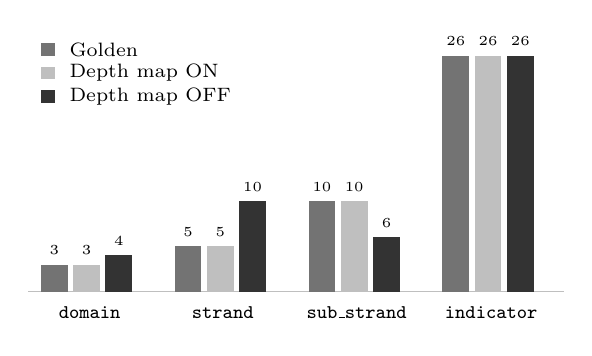
\begin{tikzpicture}[x=1cm, y=1cm]
\draw[gray!50] (0,0) -- (6.80,0);
\fill[black!55] (0.16,0) rectangle (0.50,0.346);
\node[font=\tiny, anchor=south] at (0.33,0.346) {3};
\fill[black!25] (0.57,0) rectangle (0.91,0.346);
\node[font=\tiny, anchor=south] at (0.74,0.346) {3};
\fill[black!80] (0.98,0) rectangle (1.32,0.462);
\node[font=\tiny, anchor=south] at (1.15,0.462) {4};
\node[font=\scriptsize, anchor=north] at (0.78,-0.06) {\texttt{domain}};
\fill[black!55] (1.86,0) rectangle (2.20,0.577);
\node[font=\tiny, anchor=south] at (2.03,0.577) {5};
\fill[black!25] (2.27,0) rectangle (2.61,0.577);
\node[font=\tiny, anchor=south] at (2.44,0.577) {5};
\fill[black!80] (2.68,0) rectangle (3.02,1.154);
\node[font=\tiny, anchor=south] at (2.85,1.154) {10};
\node[font=\scriptsize, anchor=north] at (2.47,-0.06) {\texttt{strand}};
\fill[black!55] (3.56,0) rectangle (3.90,1.154);
\node[font=\tiny, anchor=south] at (3.73,1.154) {10};
\fill[black!25] (3.97,0) rectangle (4.31,1.154);
\node[font=\tiny, anchor=south] at (4.14,1.154) {10};
\fill[black!80] (4.38,0) rectangle (4.72,0.692);
\node[font=\tiny, anchor=south] at (4.55,0.692) {6};
\node[font=\scriptsize, anchor=north] at (4.17,-0.06) {\texttt{sub\_strand}};
\fill[black!55] (5.26,0) rectangle (5.60,3.000);
\node[font=\tiny, anchor=south] at (5.43,3.000) {26};
\fill[black!25] (5.67,0) rectangle (6.01,3.000);
\node[font=\tiny, anchor=south] at (5.84,3.000) {26};
\fill[black!80] (6.08,0) rectangle (6.42,3.000);
\node[font=\tiny, anchor=south] at (6.25,3.000) {26};
\node[font=\scriptsize, anchor=north] at (5.88,-0.06) {\texttt{indicator}};
\fill[black!55] (0.16,3.00) rectangle (0.34,3.16);
\node[font=\scriptsize, anchor=west] at (0.40,3.08) {Golden};
\fill[black!25] (0.16,2.70) rectangle (0.34,2.86);
\node[font=\scriptsize, anchor=west] at (0.40,2.78) {Depth map ON};
\fill[black!80] (0.16,2.40) rectangle (0.34,2.56);
\node[font=\scriptsize, anchor=west] at (0.40,2.48) {Depth map OFF};
\end{tikzpicture}
\caption{Elements emitted per hierarchy level on Kentucky, whose detector golden is the corpus's only \emph{detection-exhaustive} one, with the depth-map pass enabled and ablated. With the pass enabled the detector reproduces the golden distribution exactly. Ablated, it emits an extra domain, doubles the strand count and loses four sub-strands, while the indicator count is untouched --- the failure is level \emph{collapse} at the two levels whose identity is positional rather than typographic. \textbf{This is not visible in a level-confusion matrix}: the evaluation matcher pairs on level, so an element emitted at the wrong level is recorded as a miss rather than an off-diagonal entry, and both arms render as clean diagonals. \texttt{\_only\_subset} corpus tier.}
\label{fig:levels}
\end{figure}


The mechanism is visible in Kentucky (Figure~\ref{fig:levels}), whose golden
annotates 3~domains, 5~strands, 10~sub-strands and 26~indicators. The on arm
reproduces that distribution exactly and the off arm emits 4, 10, 6 and 26.
Three repeated runs per arm show the same shape every time. Those repeats were
recorded at an earlier version of the detector code, before the Pass-1 sampler
was replaced, which is why I keep them distinct from the single-run columns of
Table~\ref{tab:ablation-depthmap}. In them the on arm reproduces the golden
distribution in all three, while the off arm inflates strand and deflates
sub-strand in all three (5~$\rightarrow$~8/7/10 and 10~$\rightarrow$~7/9/6) and
leaves the indicator count at 26. The failure is level \emph{collapse}, and it
is legible in the regression cases: with the map off, elements printed as
\texttt{Benchmark N.N} are promoted to strand, classified by their label rather
than by their position, which is precisely the behavior the method exists to
avoid.

Two qualifications. First, \textbf{the effect is conditional, not
uniform}: only Colorado and Kentucky lose recall, while Texas and Nevada keep
recall 1.000 and lose \emph{code} accuracy instead (Texas 8/8~$\rightarrow$~5/8
on an identical set of detections). Arizona and California are insensitive on
every metric, but that is an artifact of their goldens rather than a result:
both are small spot checks against far larger detection sets, so recall
saturates either way, and they are the states least able to show the effect.
Second, \textbf{off-arm recall is a range, never a point value}: across three
runs per arm per state at the earlier code version, Colorado spans 0.71--0.86
and Kentucky 0.89--0.98, and the recorded run at the current version (0.86 and
0.89) falls inside both ranges. The
direction never reverses in any sample, and the on arm is 1.000 with zero
variance across all eighteen runs, but the magnitude on any single run is a
draw. One regression case that failed at $n{=}2$ passed at $n{=}3$; I report it
as unstable rather than as evidence.

\subsection{Comparison: A Rule-Based Structure Extractor}
\label{sec:experiments-baseline}

To quantify what the language model contributes, I compare against a
rule-based structure extractor built on the cues such documents actually
provide: numbering patterns, capitalization, indentation and line shape. It is
graded by the same suite against the same goldens, through the same code path,
so the two columns are directly comparable. It was developed against the four
development states with the held-out pair untouched, and it carries no
per-document branch.

% AUTO-GENERATED by paper/analysis/generate_tables.py -- do not hand-edit.
% Source: paper/results/task4_20260823/baseline_comparison.json
% Regenerate with: python paper/analysis/generate_tables.py
% Corpus tier (guardrail 1): every row is the _only_subset tier, never full-document.
\begin{table*}
  \centering
  \begin{tabular}{lrrrrrrr}
    \hline
    & \multicolumn{2}{c}{\textbf{Recall}} & \multicolumn{2}{c}{\textbf{Raw precision}} & \multicolumn{2}{c}{\textbf{Code acc.}} & \\
    \textbf{State} & \textbf{LLM} & \textbf{Rule} & \textbf{LLM} & \textbf{Rule} & \textbf{LLM} & \textbf{Rule} & \textbf{Rule: found, wrong level} \\
    \hline
    AZ & 100.0 & 80.0 & 41.7 & 50.0 & 4/4 & 3/3 & 0/5 \\
    CA & 100.0 & 64.0 & 20.5 & 18.2 & 25/25 & 16/16 & 0/25 \\
    CO & 100.0 & 57.1 & 16.7 & 8.2 & 7/7 & 4/4 & 1/7 \\
    TX & 100.0 & 62.5 & 32.0 & 13.5 & 8/8 & 4/5 & 1/8 \\
    NV & 100.0 & 6.5 & 86.8 & 16.7 & 44/46 & 1/3 & 0/46 \\
    KY & 100.0 & 29.5 & 100.0 & 100.0 & 44/44 & 13/13 & 0/44 \\
    \hline
    \multicolumn{8}{l}{\emph{Pooled recall by level, all six states}} \\
    \hline
    domain & 100.0 & 100.0 & \multicolumn{5}{l}{LLM 13/13, rule-based 13/13} \\
    strand & 100.0 & 24.0 & \multicolumn{5}{l}{LLM 25/25, rule-based 6/25} \\
    sub\_strand & 100.0 & 66.7 & \multicolumn{5}{l}{LLM 24/24, rule-based 16/24} \\
    indicator & 100.0 & 13.7 & \multicolumn{5}{l}{LLM 73/73, rule-based 10/73} \\
    \hline
  \end{tabular}
  \caption{Rule-based baseline versus the LLM detector, graded by the \emph{same} suite against the \emph{same} goldens (Table~\ref{tab:detector-headline}). The baseline is document-agnostic: numbering depth, structural label words, ALL-CAPS and font-size cues from the bounding boxes, and column-aware reading order. It was developed against the four golden states only; NV and KY were first scored in the recorded run. \textbf{Raw precision is shown for both arms and is not a quality measure} except for KY, whose golden is detection-exhaustive: elsewhere it tracks annotation coverage, and it rewards under-emission, which is why the rule-based arm can exceed the LLM on AZ while finding fewer elements. Verified precision is not compared at all: the false-positive audit asks whether a title appears in the source text, and a rule-based extractor copies text rather than inventing it, so it scores near 1.000 by construction (\S\ref{sec:discussion-limitations}). A post-hoc probe widening two of the baseline's patterns to admit token shapes only the held-out documents use recovers NV 6.5\%$\rightarrow$52.2\%, KY 29.5\%$\rightarrow$40.9\%; the widenings are \emph{not} adopted, since they were motivated by the held-out set itself. Even repaired, the rule-based arm does not approach the LLM's recall. All numbers are on the \emph{\_only\_subset} corpus tier (8--15pp manually trimmed subsets), never full documents. Source: \texttt{paper/results/task4\_20260823/}.}
  \label{tab:baseline-comparison}
\end{table*}


\textbf{The per-level row is the result.} The rule-based arm ties the language
model exactly at domain (13 of 13 in both) and then collapses: strand
0.240, sub-strand 0.667, indicator 0.137, against 1.000 at every level. Reported
as a mean this would read ``1.000 versus 0.500'' and would hide the only thing
worth knowing. Typography identifies a document's top division in all six
states and identifies nothing reliably below it, because below the top division
the distinctions are positional.

The failure is also not the one I expected: elements the baseline misses are
overwhelmingly \emph{never emitted at all} rather than emitted at the wrong
level (43 of Nevada's 46 and 31 of Kentucky's 44). The rules do not mislabel
the structure so much as fail to see it.

\textbf{The held-out collapse needs its repair attached.} Nevada at 0.065 is the
most dramatic number in the table and the least trustworthy as stated: it is
dominated by a single token shape (\texttt{SS.ID.PK1}, a multi-letter code
segment) that none of the four development documents prints. Widening the
pattern after the fact recovers 0.522, and a comparable repair takes Kentucky
from 0.295 to 0.409. I adopt neither, because both were motivated by inspecting
held-out documents after the recorded run. The claim that survives the repair is
the one worth making: rules encode the shapes their author has seen, and even
generously repaired they reach roughly half the language model's recall on
documents they were not written against.

\textbf{Two cautions about the precision columns.} Raw precision is not a
quality ordering here: Arizona shows the rule-based arm \emph{above} the
language model (0.500 versus 0.417) purely because it emits fewer in-scope
detections against a five-element spot-check golden. I also omit verified
precision from this table deliberately. It asks whether a detected title
appears in the source text, a test for \emph{invention}, and an extractor that
copies verbatim cannot invent, so the baseline scores 1.000 in five of six
states against the language model's 0.9966. That number is real and
substantively backwards. Finally, the baseline has no Pass~1, so its depth-map
column reads \textsc{ablated} rather than failed, and it is deterministic, so
one run suffices.

\subsection{Comparison: A Single Whole-Document Prompt}
\label{sec:experiments-wholedoc}

The rule-based extractor of \S\ref{sec:experiments-baseline} answers what a
regular-expression approach cannot do. It does not answer the other obvious
question: why not hand the model the entire document in one prompt and read the
JSON back? \S\ref{sec:method-two-stage} argues against that; this measures it.
The arm is one call per document over the whole extraction, with no Pass-1 depth
map, no chunking and therefore no merge, and none of the deterministic repairs
of \S\ref{sec:method-parsing}. The prompt body, model, temperature, extractions
and grader are identical to the full method's, so a difference is attributable
to the architecture rather than to prompting.

\textbf{It is not a strawman: on Arizona and Nevada it matches}, at recall
$1.000$ with full code accuracy, and Nevada is one of the two held-out states
and prints a namespace that skips a level, so this is not an easy case. Where it
loses, it loses in two distinct ways. On Kentucky and Texas recall holds while
code accuracy falls, $44/44$ to $28/44$ and $8/8$ to $5/8$, and the failures are
precisely the repairs' absence: the model sampling its own abbreviation rule,
and codes left unanchored to their parents. Since a code composes the
identifier, each is a different primary key for the same standard. On Colorado
recall itself falls to $0.429$, with the level-collapse signature the depth-map
ablation produces.

\textbf{California is lost entirely, and that failure is architectural rather
than statistical.} Its single call emitted exactly 16{,}000 output tokens, the
configured maximum, truncating the JSON mid-object so that nothing parsed
and \emph{none} of its 25 golden elements were recovered, against $25/25$ for
the full method. One prompt has one output budget for an entire document, so
exceeding it loses the document; chunking bounds the same overflow to a chunk.
Arizona shows how narrow the margin is: it succeeded while emitting 14{,}292
tokens, within 11\% of the same ceiling, so a success here does not predict the
next document, and the margin is invisible in the score.

Scope bounds what this carries. Every subset extraction is between 3.7K and 7.9K
tokens and fits in one prompt, so a good score here would mean the architecture
is unnecessary \emph{at this tier} and would say nothing about the tiers where a
document does not fit and chunking is not optional. This arm is a single draw
per state, which is why I do not tabulate it; the California result is reported
with more confidence than the rest because its mechanism is identified rather
than inferred, the output length equaling the configured cap exactly. Source:
\texttt{task10\_20260905}.

\subsection{What the Confidence Score Measures}
\label{sec:experiments-confidence}

The detector emits a confidence score on every element, and nothing in the
pipeline thresholds it (\S\ref{sec:method-confidence}). This subsection reports
why I consider that the right decision rather than an oversight. The full
distribution, by state and by level, is
Table~\ref{tab:confidence-distribution} in
Appendix~\ref{sec:appendix-confidence}.

\textbf{The distribution is degenerate.} Across 379 elements the score takes
just five distinct values (0.90, 0.92, 0.95, 0.96 and 0.97), and 94.2\% of
them fall at 0.95 or above. The band the prompt explicitly reserves for a guess
($<0.70$) is never used once, and the whole of the range below 0.80 is empty. A
score that never exercises two thirds of the interval it was given is not
carrying much information about difficulty, and a review gate built on it would
mostly be a gate on noise.

\textbf{What variation there is tracks the document, not the difficulty of the
passage.} Three of the six states contain no sub-0.95 element whatsoever, and of
the 22 elements in the middle band, 16 belong to Kentucky alone; at indicator
level, 246 of 263 score 0.95 or above and all 17 exceptions come from two
states. Nor is the quantity stable between runs: on an earlier freeze of the
same corpus under the same configuration, 89.7\% of indicators scored 0.95 or
above against 93.5\% here, a four-point swing on an unchanged corpus, wider
than most of the distinctions a review threshold would be asked to draw.
Kentucky makes the point sharply, because it is the state I can say the most
about: its detector golden is the corpus's only exhaustive one, and against it
Kentucky achieves recall, code accuracy and verified precision of 1.000 while
carrying the lowest mean confidence of any state. Confidence separates Kentucky
from California; correctness does not.

\textbf{One observation that should not be over-read.} The single confirmed
hallucination in the corpus is also its lowest-scoring element, the only one
at 0.90, with nothing correct below 0.92, and it holds that position across
recordings. It is tempting to present this as a working detector for
fabrication. It is not one. There is exactly \emph{one} distinct invented
element in the audited corpus, so the false-negative rate of any such cut is
unmeasurable here; the threshold the prompt itself defines would catch nothing;
and the score is blind to the corpus's other non-verbatim category, since all 39
real-but-split titles, produced by column interleaving rather than by the model,
score at or above 0.95. I report the observation and decline to build on it.

\subsection{Stability: What Changes Between Identical Runs}
\label{sec:experiments-stability}

Every number reported so far is a single run of a sampling model, so the
question a reader should ask is how much of it survives re-running. I ran the
detector five times and the parser six times per state on identical frozen
inputs with caching disabled, deliberately split across two days.

% AUTO-GENERATED by paper/analysis/generate_tables.py -- do not hand-edit.
% Source: paper/results/task5_20260830/stability_analysis.json
% Regenerate with: python paper/analysis/generate_tables.py
% Corpus tier (guardrail 1): every row is the _only_subset tier, never full-document.
\begin{table}[t]
\centering
\small
\begin{tabular}{lrrr}
\toprule
& \textbf{ids} & \textbf{unstable} & \textbf{rate} \\
\midrule
\multicolumn{4}{l}{\emph{Detector}} \\
\quad AZ & 67 & 3 & 0.0448 \\
\quad CA & 51 & 0 & 0.0000 \\
\quad CO & 61 & 0 & 0.0000 \\
\quad TX & 33 & 0 & 0.0000 \\
\quad NV & 48 & 2 & 0.0417 \\
\quad KY & 44 & 0 & 0.0000 \\
\quad \textbf{pooled} & \textbf{304} & \textbf{5} & \textbf{0.0164} \\
\midrule
\multicolumn{4}{l}{\emph{Parser}} \\
\quad AZ & 45 & 0 & 0.0000 \\
\quad CA & 33 & 4 & 0.1212 \\
\quad CO & 48 & 0 & 0.0000 \\
\quad TX & 25 & 0 & 0.0000 \\
\quad NV & 24 & 5 & 0.2083 \\
\quad KY & 26 & 0 & 0.0000 \\
\quad \textbf{pooled} & \textbf{201} & \textbf{9} & \textbf{0.0448} \\
\bottomrule
\end{tabular}
\caption{Run-to-run stability, \textbf{\texttt{\_only\_subset} corpus tier}. Five detector runs and six parser observations per state, all \texttt{-{}-no-cache}, split across two days. \emph{ids} is the number of distinct element identities compared, \emph{unstable} how many differed in any graded field. \textbf{These rates are lower bounds, not estimates} (\S\ref{sec:experiments-stability}). Source: \texttt{paper/results/task5\_20260830/}.}
\label{tab:stability}
\end{table}


\textbf{The instability is concentrated rather than diffuse.} Four of six
states reproduce perfectly on each suite: California, Colorado, Texas and
Kentucky show zero detector disagreements across five runs, and Arizona,
Colorado, Texas and Kentucky zero parser disagreements across six. The movement
that exists is confined to three places, and each is a mechanism I can name.
Arizona's detector alternates on whether it emits three of its sub-strands
(present in four runs, absent in one), which changes output size without
touching any graded element. California's parser intermittently leaves the structural label inside
an indicator code, emitting \texttt{ELD.1.0.VOCA.Foundation 1.1.BROA} in two of
five comparisons. Nevada moves on both suites: a domain code that drifts between
the document's \texttt{S} and the domain's full name \texttt{Science}, and a strand
attachment that changes which of two headings three standards hang from.

\textbf{The California case is caught rather than stored.} All twelve of
those malformed codes contain whitespace, so the shape check at the validation
boundary (\S\ref{sec:method-parsing}) rejects every one before persistence. This
is the clearest evidence available that the check is load-bearing rather than
defensive decoration: the defect it was written for fires at a few percent per
run, and when it fires the records do not reach the database.

\paragraph{Why the runs were split across days.} Repeated runs inside one
session understate variance, and this measurement demonstrates it directly.
Nevada's detector emitted the same set of 54 elements in each of the three runs
executed in one evening (one of them differing only in the Science domain's
code), then dropped one indicator in \emph{both} runs executed the following
day. Five back-to-back runs would have reported that element as
perfectly stable.

\paragraph{A single run is not a safe basis for a claim, and I found that the
hard way.} An earlier recording of this system measured Nevada's detector code
accuracy at $46/46$ and I reported it as a held-out gain. It does not
reproduce: five fresh runs on identical code, the same extraction and the same
golden give $44$, $45$, $44$, $44$, $44$. Nevada's code accuracy is properly
reported as a \emph{range} of 44--45 of 46, and the earlier point value was the
top of its distribution rather than its center.

The same caution applied to a single-run ablation arm of my own, and repeating
it at $n{=}5$ per arm \emph{retired} the claim rather than confirming it. I had
attributed Nevada's two domain-code failures to the Pass-1 sampler on one draw
per arm; across five draws, one of those codes fails in \emph{every} draw of
\emph{both} arms, and at $n{=}1$ that arm had simply drawn the $46/46$ run
above. What survives is a rate rather than a cause: the layout-stratified
sampler gives mean code accuracy $0.965$ against the stride sampler's $0.935$,
its worst draw beating the stride sampler's best. But it also drops a golden
element in two draws of five where the stride sampler drops none, so it is
better on average and not better in every respect. Neither the sampler's
motivating evidence nor the depth-map ablation is affected: the first is a far
larger failure elsewhere, a four-level document reported as three
(\S\ref{sec:method-detection}), and the second is three runs per arm across six
states whose direction never changes sign.

\paragraph{What this does and does not license.} These rates are \textbf{lower
bounds, not estimates}. A defect firing in a minority of runs survives five
clean draws comfortably. The California defect above appears in two of five
comparisons, and an earlier investigation of a different parser defect, the
bare indicator code of \S\ref{sec:method-parsing}, found it in one graded run
of six within a single invocation and in ten of twenty cached runs across code
versions. A zero in Table~\ref{tab:stability} means I did not
observe instability at $n{=}5$, not that the component is deterministic. This is
why the table reports denominators beside every rate, and why the pipeline's
correctness argument rests on the validation boundary rather than on the model
agreeing with itself.

\subsection{Scale: the Batched Path on Multi-Batch Documents}
\label{sec:experiments-scale}

Every quality measurement above is computed at the \texttt{\_only\_subset}
tier, where each document produces at most five chunks and three domains. Both
batching layers therefore collapse to a single batch, the Step Functions
\texttt{Map} runs one iteration, and the merge is a no-op, so those tables,
whatever else they show, cannot support a claim about batching. This subsection
reports the one measurement that can.

% AUTO-GENERATED by paper/analysis/generate_tables.py -- do not hand-edit.
% Source: paper/results/task6_20260830/manifest.json
% Regenerate with: python paper/analysis/generate_tables.py
% Corpus tier (guardrail 1): every row is the _trimmed tier -- a document's standards content IN FULL (KY 52pp, CO 41pp) with non-standards matter removed. NOT the full published PDF (KY 120pp, CO 187pp), and NOT the _only_subset tier the quality tables use.
\begin{table}[t]
\centering
\small
\setlength{\tabcolsep}{4pt}
\begin{tabular}{lrr}
\toprule
& \textbf{KY} & \textbf{CO} \\
\midrule
Pages processed & 52 & 41 \\
\midrule
\multicolumn{3}{l}{\emph{Batching}} \\
Detection chunks & 18 & 17 \\
Detection batches & 4 & 4 \\
Parse batches & 9 & 9 \\
Elements, raw $\rightarrow$ merged & 363 $\rightarrow$ 329 & 390 $\rightarrow$ 300 \\
\midrule
\multicolumn{3}{l}{\emph{Input tokens}} \\
\quad Depth map & 12,153 & 19,613 \\
\quad Detection & 201,574 & 223,276 \\
\quad Parsing & 164,783 & 147,315 \\
\quad \textbf{Total} & \textbf{378,510} & \textbf{390,204} \\
\midrule
\multicolumn{3}{l}{\emph{Output tokens}} \\
\quad Depth map & 438 & 415 \\
\quad Detection & 64,530 & 47,125 \\
\quad Parsing & 85,205 & 83,862 \\
\quad \textbf{Total} & \textbf{150,173} & \textbf{131,402} \\
\midrule
LLM calls & 45 & 45 \\
Wall clock & 13m19s & 9m52s \\
\midrule
\multicolumn{3}{l}{\emph{Cost (USD)}} \\
\quad Depth map & \$0.0143 & \$0.0217 \\
\quad Detection & \$2.6211 & \$2.2945 \\
\quad Parsing & \$1.7724 & \$1.6999 \\
\textbf{Total} & \textbf{\$4.41} & \textbf{\$4.02} \\
\bottomrule
\end{tabular}
\caption{Batched-path scale, \textbf{\texttt{\_trimmed} corpus tier} --- each document's standards content \emph{in full}, and the only table here not at the \texttt{\_only\_subset} tier (\S\ref{sec:experiments-scale}). Each stage runs on the model assigned in \S\ref{sec:method-model-assignment}. \textbf{Tokens are the primary measure}; cost is derived from them at published Bedrock on-demand rates, recomputed at table-build time from the pipeline's own pricing constants. The depth-map pass is 0.3--0.5\% of a run's cost, detection 57--59\%. Source: \texttt{task6\_20260830}.}
\label{tab:scale}
\end{table}


\textbf{Table~\ref{tab:scale} is not the subset tier, and the distinction is
easy to misread in both directions.} These runs are the \texttt{\_trimmed}
tier: each document's standards content in full, with front matter, expository
essays and appendices removed. Kentucky's 52 pages are all of Kentucky's
standards, not 43\% of them. What the tier reduces is page count, and therefore
cost; it does not reduce coverage. Equally, these are not numbers for the
published PDFs, and the token and latency figures should not be extrapolated to
them.

At this tier the batching path is genuinely exercised: 18 and 17 detection
chunks resolve into four \texttt{Map} iterations per run, parsing into nine
batches, and the merge removes 34 and 90 duplicate elements respectively. A
no-op merge cannot remove 90 elements, so the reconciliation the architecture
performs is doing real work rather than passing data through.

\textbf{The stage breakdown is where the model-assignment principle of
\S\ref{sec:method-model-assignment} is tested.} Detection is the only stage
invoked once per chunk and accounts for 57--59\% of each run's cost. The
depth-map pass, the component the ablation above shows carries the
intermediate levels, runs once per document on the cheapest model and costs
between 0.3\% and 0.5\% of a run, about 1.4 cents on Kentucky and 2.2 on
Colorado. The most load-bearing
component in the method is very nearly the cheapest one, which is the outcome
the assignment was designed for.

Tokens are the primary measure and cost is derived from them at published
on-demand rates, recomputed at table-build time from the pipeline's own pricing
constants rather than transcribed by hand. Neither run was throttled, no
detection chunk returned empty, and the validator rejected no records, so these
figures describe a clean pass rather than a degraded one.

\subsection{Quality at Full-Document Scale}
\label{sec:experiments-scale-quality}

Every quality figure above is computed at the \emph{\_only\_subset} tier, and
the obvious objection is that subset-tier quality may not survive a whole
document: a larger run chunks further, and chunk boundaries are where a
detector can duplicate an element or lose one. \S\ref{sec:experiments-scale}
establishes that the batching path is genuinely exercised at the
\emph{\_trimmed} tier but grades nothing. This subsection grades it.

% AUTO-GENERATED by paper/analysis/generate_tables.py -- do not hand-edit.
% Source: paper/results/task13_20260907/ky_trimmed_3runs.json
% Regenerate with: python paper/analysis/generate_tables.py
% Corpus tier (guardrail 1): every row is the _trimmed tier -- a document's standards content IN FULL (KY 52pp, CO 41pp) with non-standards matter removed. NOT the full published PDF (KY 120pp, CO 187pp), and NOT the _only_subset tier the quality tables use.
\begin{table}[t]
\centering
\small
\setlength{\tabcolsep}{4pt}
\begin{tabular}{lrrrr}
\toprule
& \textbf{1} & \textbf{2} & \textbf{3} & \textbf{sd} \\
\midrule
\multicolumn{5}{l}{\emph{Detector} --- 277 verified elements} \\
\quad Elements emitted & 328 & 327 & 328 & 0.6 \\
\quad Absent from run & 0 & 0 & 0 & 0.0 \\
\quad Hallucinations & 0 & 0 & 0 & 0.0 \\
\quad Recall (level+title) & 1.000 & 1.000 & 1.000 & 0.000 \\
\quad Recall (strict key) & 0.592 & 0.588 & 0.592 & 0.002 \\
\quad Spurious \texttt{age\_band} & 164 & 164 & 164 & 0.0 \\
\quad Surplus duplicates & 51 & 50 & 51 & 0.6 \\
\midrule
\multicolumn{5}{l}{\emph{Parser} --- 207 verified standards} \\
\quad Standards parsed & 214 & 220 & 220 & \\
\quad Coverage & 0.807 & 0.927 & 0.841 & 0.062 \\
\quad Field accuracy & 0.997 & 0.994 & 0.994 & 0.002 \\
\quad Fabricated \texttt{.N} keys & 10 & 11 & 11 & 0.6 \\
\quad Collisions$^{\dagger}$ & 0 & 0 & 0 & 0.0 \\
\bottomrule
\end{tabular}
\caption{Quality at whole-document scale: Kentucky, three independent runs, \textbf{\texttt{\_trimmed} corpus tier} --- the document's standards content \emph{in full}, and not the \texttt{\_only\_subset} tier every other quality table uses (\S\ref{sec:experiments-scale-quality}). \textbf{Recall is measured against a verified reference set, not against the document}, so an element no run emits is invisible here (\S\ref{sec:discussion-goldens}). \textbf{Coverage is a range and must not be read as its mean.} $\dagger$~zero by construction: the resolver renames every collision before the check runs, so the informative count is the fabricated-key row above. Source: \texttt{task13\_20260907}.}
\label{tab:scale-quality}
\end{table}


\paragraph{Two measurements, and why the second was necessary.} The first
regrades the existing \emph{\_only\_subset} goldens \emph{inside} the
trimmed-tier run, translating page numbers through the recorded page map of
\S\ref{sec:corpus}. It needs no new annotation, and it isolates the variable
that matters: the same pages, the same golden, a larger neighborhood. Kentucky
and Colorado both come back with zero elements absent and zero ungrounded
detections. That measurement cannot speak to the rest of the document, so a
second one was built: both Kentucky trimmed-tier goldens are new (277
detected elements and 207 normalized standards, seeded from one recorded run
and then checked page by page against the published PDF), and three further
runs were executed and graded against them (Table~\ref{tab:scale-quality}).
Because the goldens were verified against a document rather than against the
run being graded, a miss is a real miss.

\paragraph{Detection recovers the whole reference set at scale.} All \textbf{277 of 277} verified
elements are found by all three runs. Not one is missed, and not one ungrounded
element is emitted, across a $6.5\times$ increase in page count and four
detection batches per run.

\paragraph{One field accounts for every anomaly.} Kentucky prints a
\texttt{THREE AND FOUR YEAR OLDS} banner at the head of each page. At the subset
tier the detector ignores it and every element comes back with a null age band,
matching the golden. At the trimmed tier it does not: 164 elements carry the
banner as their own \texttt{age\_band} in each of the three runs, with a
standard deviation of zero on the count, and 159 of those elements are the
same in all three runs (two runs agree exactly; the third differs on five). That
makes this a \textbf{systematic misreading rather than sampling noise}. Three
consequences follow, and together they are the entire difference between the
strict figures in Table~\ref{tab:scale-quality} and the ones above:

\begin{enumerate}
  \item elements fail the evaluation's matching key on that field alone, which
    is why strict recall reads $0.59$ while recall by level and title is
    $1.000$;
  \item \texttt{\_dedup\_elements} keys on \texttt{age\_band}, so the two
    spellings of one element never merge, and roughly 15\% of detector output
    survives as surplus duplicates;
  \item those duplicates collide in parsing and are separated by the
    identifier resolver's numeric fallback, so ten to eleven fabricated primary
    keys per run reach persistence, naming standards that do not exist.
\end{enumerate}

\textbf{Colorado is the control.} Its document has no age-band column and no
such banner, and in the same measurement it produces \textbf{zero} duplicates
and zero fabricated keys over 240 standards. That contrast is what makes the
attribution a measurement rather than a hypothesis.

\paragraph{Parser coverage is a range; parser field accuracy is not.} Coverage
spans twelve points across the three runs while field accuracy holds at $0.995
\pm 0.002$. The swing tracks the dropped-standard count exactly, and the
dropped standards are those the run assigned a narrower age band than the
document carries. \textbf{A single coverage figure for this document would be a
draw from that range}, and I report all three rather than their mean.

\paragraph{Two figures that look reassuring and are not.} Identifier collisions
are zero by construction: the resolver renames every collision before any
check runs, so the informative count is the fabricated keys above. And recall
here is measured \emph{against a verified reference set}, not against the
document: an element that no run emits is absent from the golden too, and
invisible to this measurement (\S\ref{sec:discussion-goldens}).

\paragraph{What this establishes.} Detection quality survives full-document
scale on the one document where it can be checked: complete recovery of a
verified reference set, no hallucination, in three independent runs. The
defects that scale introduces are concentrated in one field, are systematic
rather than random, and are documented rather than repaired, because the repair
changes a prompt and would invalidate every frozen measurement in this paper
(\S\ref{sec:discussion-limitations}). Source:
\texttt{task9\_20260905} and \texttt{task13\_20260907}.
